\subsubsection{Adjusting the Camera}
In 3D animation software, there are multiple ways to accomplish the same thing. An example of this is how to position a camera in the scene. This can be done by manually adjusting the X, Y and Z position of the camera; moving it by dragging a handle tool; or, alternatively, by using the the \textit{Look Through Selected} feature \cite{maya_lookThrough}. During the initial observations, it was clear that many of the artists at The Animation Workshop preferred this feature. This concept was translated directly into the camera tool. Using the \textit{be the camera} feature (see Figure \ref{fig:beTheCam}), the artists can place their camera by navigating the scene in Unity with the \textit{Flythrough mode} \cite{unity_flyMode}.

\begin{figure}[htbp]
\centering
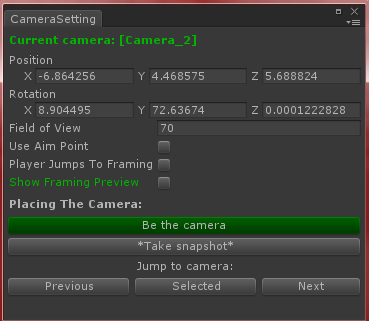
\includegraphics[width=0.3\textwidth]{Pics/be_the_cam_new}
\caption{Pressing the green button puts the user in a special mode where the selected camera inherits position and orientation data from the scene camera. To exit the mode, the user has to press the button again (which now spells "Exit the camera" in red).}
\label{fig:beTheCam}
\end{figure}

Another way to position the camera in Maya is by using an aim-vector control point \cite{maya_camAim}. The artists at The Animation Workshop used this to quickly make the camera aim at something in the scene. This concept has also been designed for the camera tool (see Figure \ref{fig:aimPoint}).

\begin{figure}[htbp]
\centering
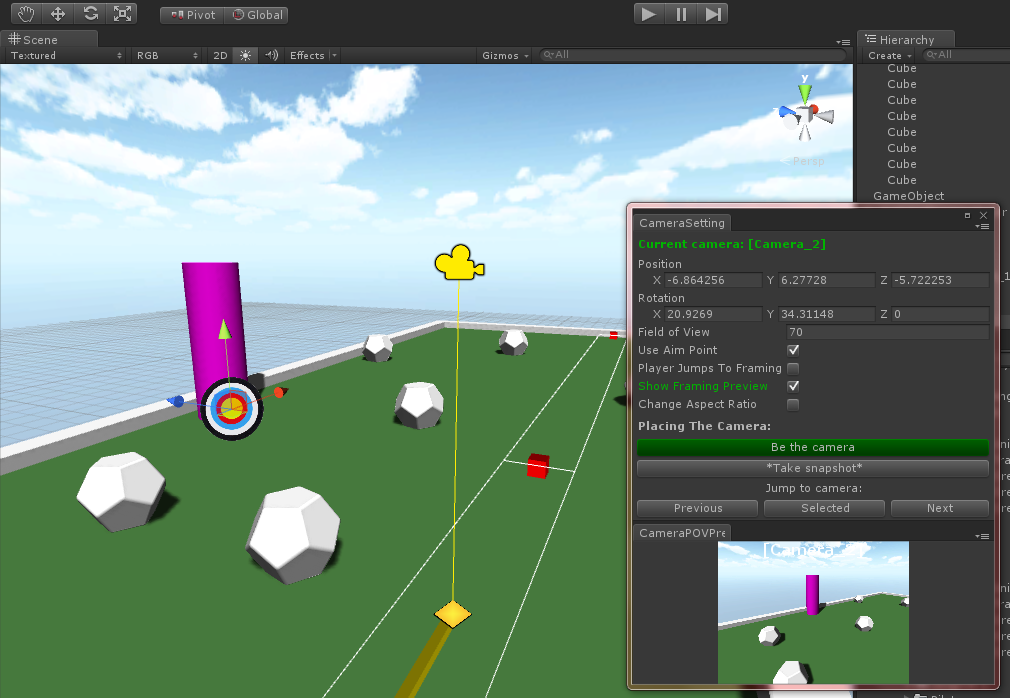
\includegraphics[width=0.3\textwidth]{Pics/aimPoint}
\caption{The aim point allows for quick adjustments of the camera.}
\label{fig:aimPoint}
\end{figure}

%It was discovered that none of the artists knew how to use a standard Unity feature that lets the player fly around with the scene camera as if they were playing a first-person game ("Flythrough Mode", \cite{unity_flyMode}). The artist were excited about the discovery of this feature. One artist perceived the standard way of moving around in Unity as confusing, while another stated that the way of moving the camera is exactly like in Maya. After testing this ourselves, we concluded that the movement controls in Maya and Unity are indeed very similar (except for the "Flythrough Mode"), which means that the artists should ideally be comfortable with navigating in either of the applications.

\subsubsection{Immediate Feedback \& Quick Preview}
An important aspect for the tool was to provide clear feedback. A common request from all of the artists were the ability to quickly preview their changes. Instead of having to start the game and navigate the player character to a specific framing, the artists wanted to quickly jump to a specific framing to test out how it feels and looks.

The artists suggested that they should be able to move the player character around in the editor. Initially, this seemed like a fine way to preview the framings. We considered this option, but deemed it a bit impractical, since it sometimes would be hard to locate the player character in a big scene. Instead, we took inspiration from Camera Path Animator 3.0 mentioned in Section \ref{relatedWork} by designing an interactive slider. With this feature, the artists are able to choose the start and end framing. By dragging the slider between those, the artists can quickly get a feel of how the camera movements will look (see Figure \ref{fig:slider}).

%\begin{figure}[htbp]
%\centering
%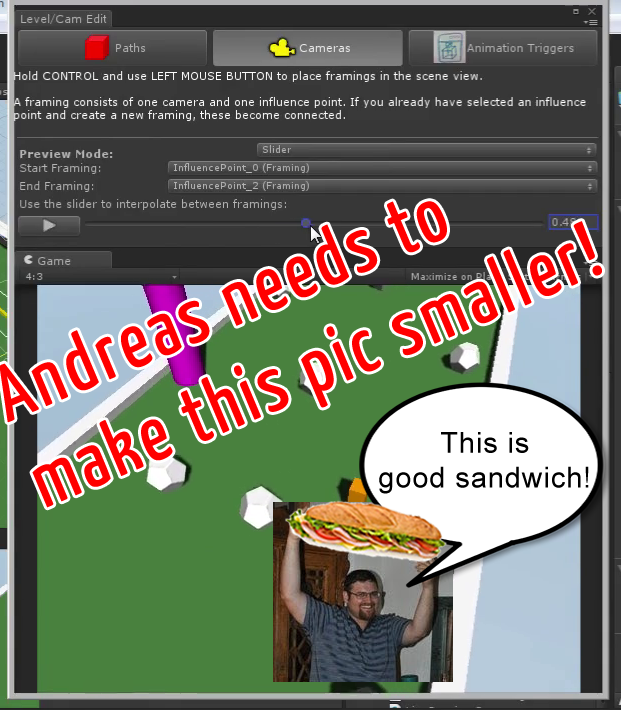
\includegraphics[width=0.3\textwidth]{Pics/slider}
%\caption{The slider provides a quick way to preview the framings.}
%\label{fig:slider}
%\end{figure}